\documentclass[12pt]{article}

% Package lists
\usepackage{listings}
\usepackage{xcolor}
\usepackage{geometry}
\usepackage{graphicx}

% Configurations here
\definecolor{codegreen}{rgb}{0,0.6,0}
\definecolor{codegray}{rgb}{0.5,0.5,0.5}
\definecolor{codepurple}{rgb}{0.58,0,0.82}
\definecolor{backcolour}{rgb}{0.95,0.95,0.92}
 
\lstdefinestyle{mystyle}{
    backgroundcolor=\color{backcolour},   
    commentstyle=\color{codegreen},
    keywordstyle=\color{magenta},
    numberstyle=\tiny\color{codegray},
    stringstyle=\color{codepurple},
    basicstyle=\ttfamily\footnotesize,
    breakatwhitespace=false,         
    breaklines=true,                 
    captionpos=b,                    
    keepspaces=true,                 
    numbers=left,                    
    numbersep=5pt,                  
    showspaces=false,                
    showstringspaces=false,
    showtabs=false,                  
    tabsize=2
}
\lstset{style=mystyle}

\geometry{margin=1cm, bottom=2cm}
\setlength{\columnseprule}{1pt}

\begin{document}
  \title{Homework 8 - Discrete Mathematics}
  \author{Nguyen Tien Duc - ITITIU18029}
  \maketitle
  \part{Finding shortest path}
    \section*{Dijkstra Algorithm}
      \lstinputlisting[language=c++]{../Dijkstra.cpp}
    \section*{Floyd Algorithm}
      \lstinputlisting[language=c++]{../Floyd.cpp}
    \section*{Main Function}
      \lstinputlisting[language=c++]{../ShortestPath.cpp}
    \section*{Demo}
    As the requirements are the same for both algorithms, so both algorithms take the same inputs and also output the same thing. \\ 
    Therefore, I only took 1 demo picture.
      \begin{center}
        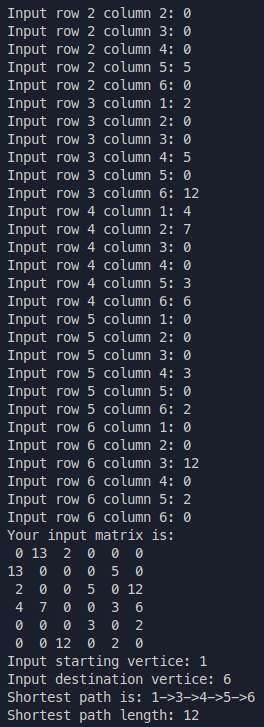
\includegraphics{../DijkstraDemo.png}
      \end{center}
    \section*{Exersize 4 / page 655}
      I solved the exercise using both algorithms.\\
      Although there is a slight difference in the path, the shortest path length is still the same.
      \subsection*{Dijkstra's Result}
        \begin{center}
          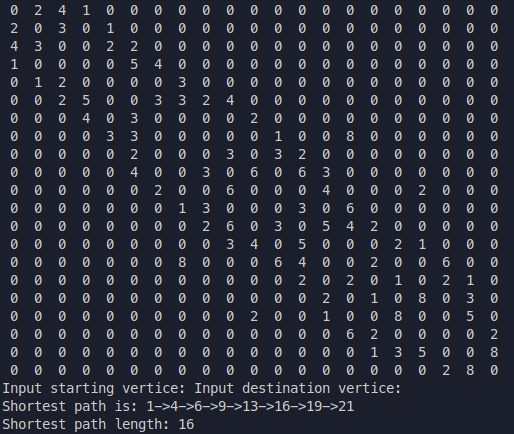
\includegraphics{../DijkstraResult.png}
        \end{center}
      \subsection*{Floyd's Result}
        \begin{center}
          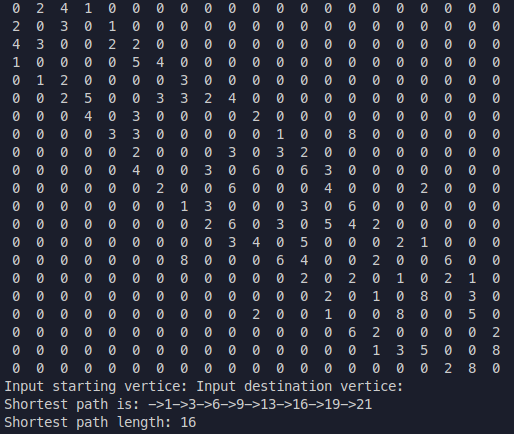
\includegraphics{../FloydResult.png}
        \end{center}
  \part{Minimum spanning tree}
    \section*{Kruskal Algorithm}
      \subsection*{Code}
        \lstinputlisting[language=c++]{../Kruskal.cpp}
      \subsection*{Demo}
\end{document}